\documentclass[
 reprint,
 amsmath,
 amssymb,
 aps,
]{revtex4-2}

\usepackage{graphicx}
\usepackage{dcolumn}
\usepackage{physics}
\usepackage{bm}
\usepackage{hyperref}

\begin{document}

\title{2D Ising Model with MCMC}

\author{Matthew Yao}
\email{mhyao@ucsd.edu}
\author{Ashleann Chen}
\email{asc05@ucsd.edu}
\author{Sophie Carlson}
\email{s1carlson@ucsd.edu}

\affiliation{
 University of California San Diego
}

\collaboration{Group: 2D Ising model with MCMC (B)}

\date{\today}

\begin{abstract}
The Ising model is a mathematical model of ferromagnetism in statistical 
mechanics. 
It consists of a lattice of spins which can be in one of two states,
spin up or spin down, and an external magnetic field $ B $.
In this project, we will use the Metropolis-Hastings algorithm to simulate the
2D Ising model and study the phase transition from a disordered to an 
ordered state.
We use Numba and NumPy to optimize our code so that each iteration
runs in $ \mathcal{O}(z) $ time, where $ z $ is the number of nearest neighbors.
This speeds up our simulation by a factor of $ 300\times $ compared to 
a naive python only implementation.
We find that there is a first order phase transition line at $ B=0 $
and $ T < T_{c} $ for varying $ B $,
and a second order phase transition at $ B=0 $ and $ T = T_{c} $
for varying $ T $.
$ T_{c} \approx 2.269 $ is the analytical critical temperature for the 
2D Ising model.

\end{abstract}

\maketitle


\section{Introduction}
\label{sec:intro}

The Ising model is a mathematical model of ferromagnetism.
It consists of a lattice of spins which can be in one of two states, 
spin up or spin down, and an external magnetic field $ B $.
The Hamiltonian for the 2D Ising model is given by 
\begin{equation}
\hat{H} = -J \sum_{\langle i,j \rangle} \sigma_{i} \sigma_{j}
- B \sum_i \sigma_{i}
\end{equation}
where $ J $ is the coupling constant, 
$ \sigma_i $ is the spin at site $ i $,
and the sum $ \langle i,j \rangle $ is over nearest neighbors.
The first sum represents the interaction between nearest neighbor spins,
and the second sum represents the interaction between spins and the external
magnetic field.
We will be using a 2D rectangular lattice of size $ 100\times 100 $ with 
periodic boundary conditions.
The statistical mechanics of the Ising model can be studied using the
canonical ensemble, where the probability of a configuration is given by the
Boltzmann factor
\begin{equation}
P(\sigma) = \frac{1}{Z} e^{-\beta \hat{H}(\sigma)}.
\end{equation}
For our configuration,
the total number of configurations is $ 2^{N^{2}} $,
which is intractable for large $ N $,
so we will use the Metropolis-Hastings algorithm to sample from the
Boltzmann distribution.
The Metropolis-Hastings algorithm is a Markov chain Monte Carlo (MCMC)
method that generates a sequence of configurations by proposing a new
configuration and accepting or rejecting it based on the change in energy.
The acceptance probability is given by
\begin{equation}
P_{acc} = \min\left(1, e^{-\beta \Delta E}\right) 
\end{equation}
where $ \Delta E = \hat{H}(\sigma') - \hat{H}(\sigma) $ 
is the change in energy
when moving from the current configuration $ \sigma $ to the proposed
configuration $ \sigma' $,
and $ \beta = \frac{1}{k_{B}T}$ is the inverse temperature.
The change in configuration per step is a randomly chosen spin flip,
so the change in energy is given by 
\begin{equation}
\Delta E = 2J \sum_{\langle i,j \rangle} \sigma_{i} \sigma_{j} + 2B \sigma 
\end{equation}

Using this algorithm, we can simulate the 2D Ising model and study how
the mean magnetization $ m $ change with temperature and the external magnetic
field. Using this information, we determine the phase transitions
and the critical points of the system.
In section \ref{sec:methods},
we describe the implementation of the Ising model and the Metropolis-Hastings
algorithm, along with the optimizations we made to speed up the simulation.
In section \ref{sec:results}, we present the results of our simulations,
including the mean magnetization as a function of temperature and the
external magnetic field, and the phase diagram of the system.
Finally, in section \ref{sec:conclusion}, we summarize our findings
and compare to the analytical results for the 2D Ising model.


\section{Methods}
\label{sec:methods}

We implement the lattice as a 2d Numpy array of size $ N\times N $,
where we choose $ N = 100 $.
Each element of the lattice represents a site,
which contains a spin of $ \sigma \in \qty{\pm 1} $.
We work with units where $ J = 1 $ and $ k_{B} = 1 $.

We use the Metropolis-Hastings algorithm to sample from the Boltzmann
distribution.
To iterate the algorithm,
we randomly select a site on the lattice and propose a new configuration
by flipping the spin at that site.
We then calculate the change in energy $ \Delta E $ using the Hamiltonian
and the current configuration.
The acceptance probability is calculated using the formula
\begin{equation}
P_{acc} = \min\left(1, e^{-\beta \Delta E}\right).
\end{equation}
This formula can be interpreted as follows:
if the change in energy is negative ($ \Delta E < 0 $),
then automatically accept the new configuration,
if the change in energy is positive ($ \Delta E > 0 $),
then accept the new configuration with probability
$ e^{-\beta \Delta E} $.
We can calculate $ \Delta E $ using the formula
\begin{equation}
\Delta E = 2J \sum_{\langle i,j \rangle} \sigma_{i} \sigma_{j} + 2B \sigma, 
\end{equation}
where the first term is the interaction energy with nearest neighbors
and the second term is the interaction energy with the external magnetic field.

We initialize the lattice with random spins, weighted by 
the external magnetic field $ B $, i.e.
the probability is given by 
\begin{equation}
p(\sigma) = \frac{e^{-\beta \sigma}}{Z}
\end{equation}
where $ Z = \Tr e^{-\beta \sigma} $ is the single site partition function.
This has the effect that the initial spins are 
biased towards the direction of the external magnetic field.
This is to ensure that we start the simulation in a state that is not too far
from the equilibrium state, which speeds up the convergence of the simulation.
We run the simulation for $ 1,000,000 $ iterations,
and we discard the first $ 200,000 $ iterations as a burn-in period.

To optimize the simulation, we use a variety of optimizations.
Instead of calculating a random site and a random number each iteration,
we calculate an array of random sites and numbers ahead of time and
use them in the simulation.
This is faster as it is faster to calculate a random array of numbers of length
$ N $ than to calculate a random number $ N $ times.
This also has the effect of working better with Numba.
We are trading off the time with space complexity,
so the space complexity to store the random numbers is 
$ \mathcal{O}(\mathrm{STEPS}) $.
From our experiments, we find that this is about $ 50\times $ faster than
computing a random number each iteration.

To calculate the mean, we store the total number of spins.
We initialize a variable to store the total number of spins at the beginning
of the simulation and update it each time we flip a spin,
instead of recalculating the total number of spins each time.
This reduces the complexity of calculating the mean from 
$ \mathcal{O}(N^{2}) $ to $ \mathcal{O}(1) $.

The most significant speed up is the use of Numba. Numba is a
just-in-time compiler for Python that translates a subset of Python and NumPy
code into fast machine code at runtime.
This, along with the optimizations above, allows us to run the simulation
in $ \mathcal{O}(z\cdot \mathrm{STEPS}) $ time, 
where in our case, $ z = 4 $, and $ \mathrm{STEPS} = 1,000,000 $.

The code can be found in the Github repository at 
\url{https://github.com/mattyaoo/phys142final}.

\section{Results}
\label{sec:results}

We simulate the 2D Ising model for various values of the external magnetic
field $ B $ and temperature $ T $.
We fix $ T $ in three cases: $ T < T_{c} $, $ T=T_{c} $, and $ T > T_{c} $,
and vary $ B $.
For each value of $ B $ and $ T $,
we compute the mean magnetization $ m $ with the MCMC simulation.

\begin{figure}[ht]
\centering
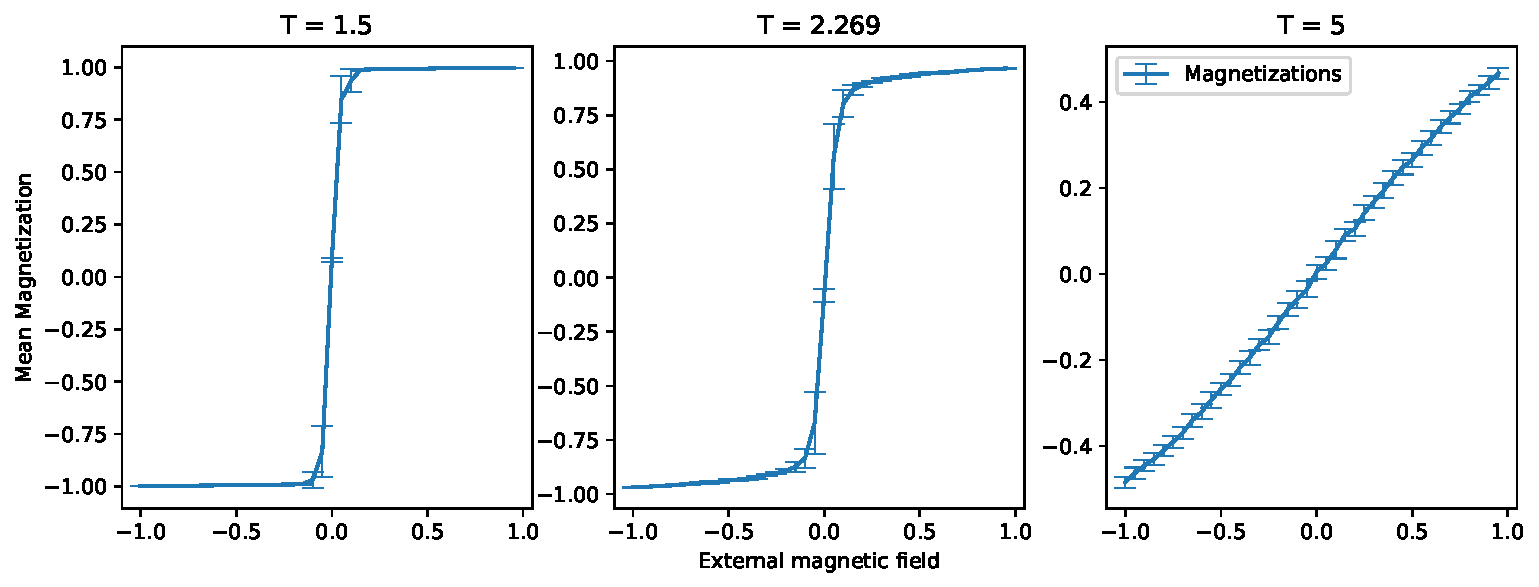
\includegraphics[width=0.5\textwidth]{figures/m_vs_B.pdf}
\caption{Mean magnetization $ m $ as a function of the external magnetic 
field $ B $}
\label{fig:m_vs_B}
\end{figure}

When $ T < T_{c} $, there is a discontinuity in the mean magnetization
as a function of $ B $.
This is an indication of a first order phase transition.
When $ T \geq T_{c} $,
the mean magnetization $ m $ is continuous as a function of $ B $,
so there is no phase transition.

Next, we fix $ B = -1, 0, 1 $, and plot $ m $ as a function of $ T $
in Figure \ref{fig:m_vs_T}.
\begin{figure}[ht]
\centering
\includegraphics[width=0.5\textwidth]{figures/m_vs_T.pdf}
\caption{Mean magnetization $ m $ as a function of temperature $ T $.}
\label{fig:m_vs_T}
\end{figure}
We see that when $ T < T_{c} $,
and $ B\neq 0 $,
the mean magnetization $ m $ is very close to $ B $.
This indicates that the system is in a ferromagnetic state,
where the spins are aligned with the external magnetic field.
When $ T > T_{c} $,
the mean magnetization trends towards zero,
indicating that the system is in a disordered state,
and no longer ferromagnetic.
The magnetization is slightly biased towards the direction of the external
magnetic field.

For $ B = 0 $, we initialized the lattice with spins slightly biased towards
spin up to show the phase transition.
When $ T < T_{c} $,
mean magnetization $ m $ is close to $ 1 $,
indicating that all the spin down states have flipped to spin up,
despite the external magnetic field being zero.
This is an indication of ferromagnetism.
When $ T $, increases past $ T_{c} $,
the mean magnetism sharply drops to zero,
indicating that the system has transitioned to a disordered state.
This is a second order phase transition, as the mean magnetization
is continuous as a function of $ T $.

We aggregrate the previous two results to create a phase diagram of the 
2D Ising model, shown in Figure \ref{fig:phase}.
For $ -1 < B < 1 $, and $ 0 < T < 10 $,
we plot the mean magnetization $ m $ as a function of $ B $ and $ T $.

\begin{figure}[ht]
\centering
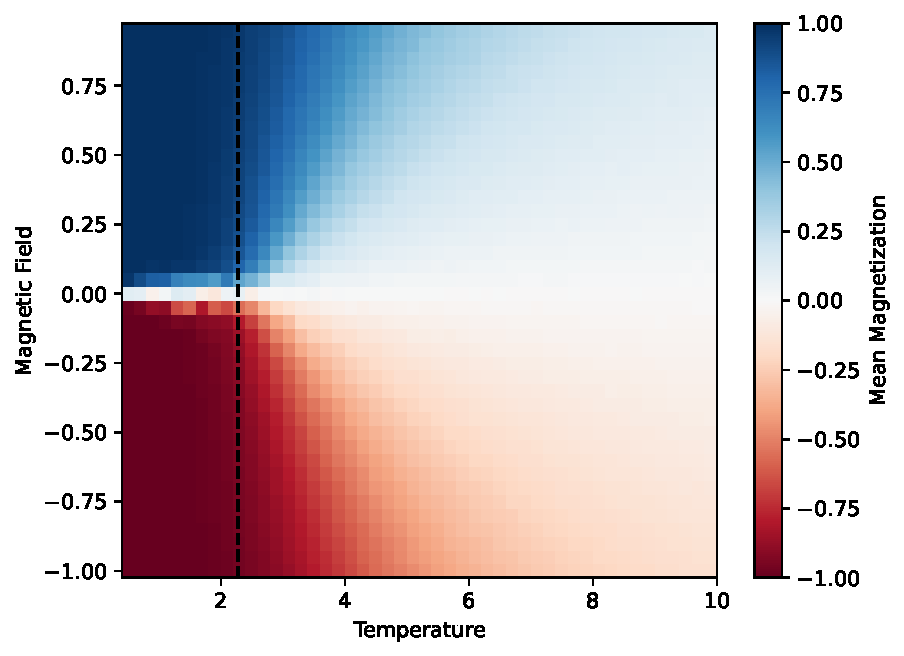
\includegraphics[width=0.5\textwidth]{figures/phase.pdf}
\caption{Phase diagram of the 2D Ising model.
The color indicates the mean magnetization $ m $, 
and the black dashed line is the analytical critical temperature.}
\label{fig:phase}
\end{figure}

We see that for $ T < T_{c} $,
there is a sharp discontinuity in the mean magnetization $ m $ 
as a function of $ B $, which is our first order phase transition.
We can see that the first order phase transition line is at $ B=0 $,
extending from $ T = 0 $ to $ T= T_{c} $.
When $ T > T_{c} $,
there is no longer a discontinuity in the mean magnetization 
as a function of $ B $.
This is the disordered state. 
We see that the mean magnetization tends towards zero as $ T $ increases,
and $ B $ decreases.

We demonstrate the hysteresis of the system by changing the external magnetic
field as a function of time.
Starting with $ B = 0 $ and $ m = 0 $,
we increase $ B $ from $ 0 $ to $ 1 $ in 1,000,000 MCMC steps,
then decrease $ B $ from $ 1 $ to $ -1 $ in 2,000,000 MCMC steps,
and finally increase $ B $ back to $ 0 $ in 2,000,000 MCMC steps.
We plot $ m $ against $ B $ in Figure \ref{fig:hysteresis}.
\begin{figure}[ht]
\centering
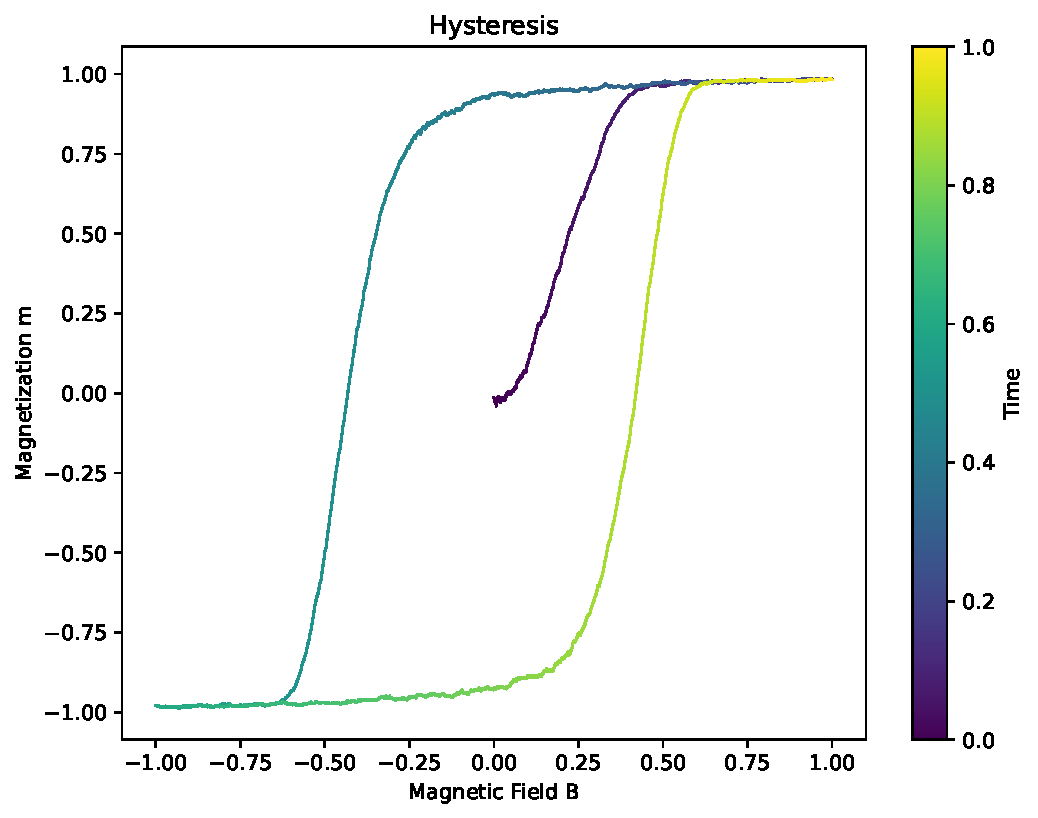
\includegraphics[width=0.5\textwidth]{figures/hysteresis.pdf}
\caption{Hysteresis of the 2D Ising model.}
\label{fig:hysteresis}
\end{figure}
The mean magnetization increases to $ 1 $ as $ B $ increases to $ 1 $,
and decreases to $ -1 $ as $ B $ decreases to $ -1 $.
Notice that the curve is different from \ref{fig:m_vs_B},
where the mean magnetization switches signs as $ B $ crosses zero.
This is an indication of hysteresis in the system,
where the mean magnetization is dependent on the history of the system.
We see that the magnet tends to stay in the same state as it was before,
which is an indication of ferromagnetism.



\section{Conclusion}
\label{sec:conclusion}
The Ising model is a well-studied model in statistical mechanics
that describes the behavior of ferromagnetic materials.
It turns out that the $ P-V $ phase diagram of gasses is topologically
equivalent to that of the $ B-T $ phase diagram of magnetization,
so studying the Ising model can give us insight into the behavior of gasses
as well.
Our exploration of the 2D Ising model gives us insights into phase
transitions and critical phenomena which are universal across many
physical systems.

In this project, we simulated the 2D Ising model using the Metropolis-Hastings
algorithm and studied the phase transitions of the system.
We found that there is a first order phase transition line at $ B=0 $
and $ T < T_{c} $ for varying $ B $, and a second order phase transition
at $ B=0 $ and $ T = T_{c} $ for varying $ T $.
We find that the critical point at $ B = 0, T = T_{c} $ agrees well with
the analytical critical temperature for the 2D Ising model.
We aggregate this information to create a phase diagram of the 2D Ising model,
which shows the mean magnetization as a function of the external magnetic
field and temperature.
We also demonstrated the hysteresis of the system by changing the external
magnetic field as a function of time,
which shows that the mean magnetization is dependent on the history of the
system.

In the future, we can extend this work to study the energy,
heat capacity, and susceptibility of the system,
which are important quantities in statistical mechanics.
We can also study metastability and critical exponents of the system.
Our initial parameters for the simulation were not varied much,
so we could also explore the effect of changing the lattice size and 
the number of steps. We could also explore 1d or 3d Ising models using the 
same methodology.


\section{Contributions}

Matthew Yao was responsible for coding the simulation, contributing to the presentation, and developing key ideas for the project. Sophie Carlson and Ashleann Chen contributed to generating ideas, contributing to the presentation, and writing the paper.


\appendix


\end{document}
